% Shared standalone design for the editable figure reconstructions.
\documentclass[tikz,border=5pt,10pt]{standalone}
\usepackage[T1]{fontenc}
\usepackage[utf8]{inputenc}
\usepackage{newpxtext,newpxmath}
\usepackage[scaled=.94]{sourcesanspro}
\usepackage{pgfplots}
\pgfplotsset{compat=1.18}
\usetikzlibrary{arrows.meta,calc,positioning,decorations.pathreplacing,
  decorations.markings,patterns,matrix,shapes.geometric,fit,backgrounds,
  intersections,angles,quotes}
\definecolor{ink}{HTML}{203746}
\definecolor{accent}{HTML}{146C78}
\definecolor{muted}{HTML}{667780}
\definecolor{signalred}{HTML}{B94B44}
\color{ink}
\tikzset{>=Latex,line width=.8pt,
  every node/.style={font=\small},
  axis/.style={->,draw=muted,line width=.5pt},
  guide/.style={draw=muted,dashed,line width=.45pt},
  curve/.style={draw=accent,line width=1pt},
  marker/.style={circle,fill=accent,inner sep=1.5pt},
  labelbox/.style={fill=white,inner sep=2pt}}

\begin{document}
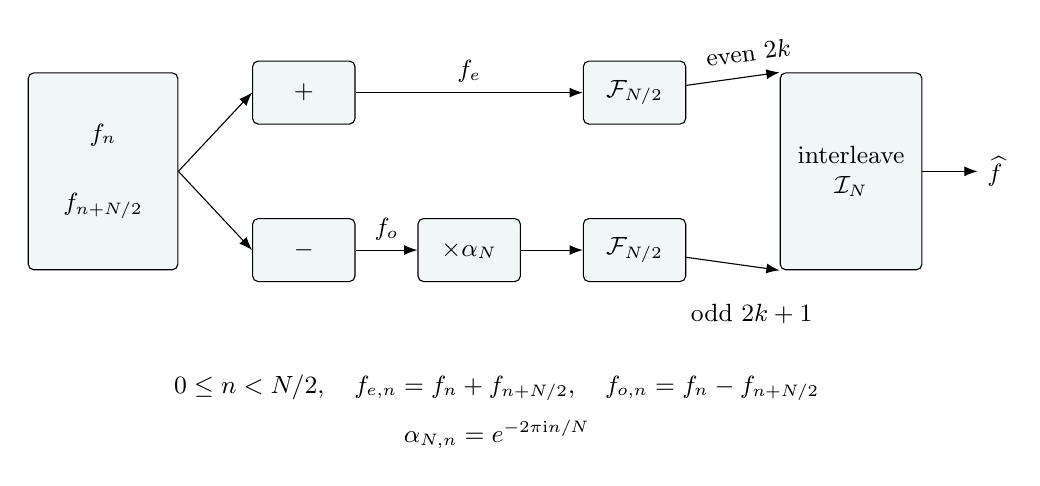
\begin{tikzpicture}[x=1cm,y=1cm,block/.style={draw,rounded corners=2pt,fill=accent!6,minimum width=1.3cm,minimum height=.8cm,align=center}]
\node[block,minimum width=1.9cm,minimum height=2.5cm] (input) at (0,0) {$f_n$\\[5mm]$f_{n+N/2}$};
\node[block] (plus) at (2.55,1) {$+$};\node[block] (minus) at (2.55,-1) {$-$};
\draw[->] (input.east)--(plus.west);\draw[->] (input.east)--(minus.west);
\node[block] (twiddle) at (4.65,-1) {$\times\alpha_N$};
\node[block] (ffta) at (6.75,1) {$\mathcal F_{N/2}$};
\node[block] (fftb) at (6.75,-1) {$\mathcal F_{N/2}$};
\draw[->] (plus)--node[above] {$f_e$}(ffta);
\draw[->] (minus)--node[above] {$f_o$}(twiddle);\draw[->] (twiddle)--(fftb);
\node[block,minimum height=2.5cm,minimum width=1.8cm] (interleave) at (9.5,0) {interleave\\$\mathcal I_N$};
\draw[->] (ffta)--node[pos=.7,above=2pt,sloped] {even $2k$}(interleave.north west);
\draw[->] (fftb)--node[pos=.7,below=10pt] {odd $2k+1$}(interleave.south west);
\draw[->] (interleave.east)--++(.7,0) node[right] {$\widehat f$};
\node[align=center] at (5,-3.05) {$0\le n<N/2,\quad f_{e,n}=f_n+f_{n+N/2},\quad f_{o,n}=f_n-f_{n+N/2}$\\[2mm]$\alpha_{N,n}=e^{-2\pi\mathrm{i}n/N}$};
\end{tikzpicture}
\end{document}
